\section{Test}

\subsection{Magnitude-tests}

For at finde ud af hvordan der kan bestemmes et fornuftigt threshold, skal der findes ud af hvorledes magnitude for DTMF-frekvenserne ændrer sig under forskellige fysiske forhold - nærmere bestemt vinklen mellem højtaler og mikrofon, afstanden mellem dem og transmissionshastigheden. Målet er at finde ud af, om der er tendenser man kan programmere threshold efter. 

\subsection{Vinduefunktioner}

Når et signal samples, kan der opstå spectral leakage, hvis signalet er ude af fase, når man kommer til sidste sample.

\begin{figure}[h]
\centering
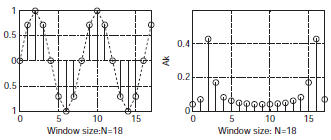
\includegraphics[scale=0.8]{Billeder/SpectralLeak.PNG}
\caption{Her kan man se at der kommer uønskede frekvenser med i signalet, fordi N er valgt så samplingen stopper et stykke inde i 3. periode}
\label{fig:Spectral}
\end{figure} 

Denne diskontinuitet (figur \ref{fig:Spectral}) tilfører støj til signalet i form a frekvenser, der egentlig ikke er til stede. Man kan mindske indflydelsen af spectral leakage ved at gange en såkaldt vinduefunktion på alle samples. Vinduet går mod 0 i enderne, og er højest midt i signalet.\\
Spectral leakage vil nødvendigvis blive et problem, når der vælges en fast mængde af samples, der kigges på til at finde forskellige frekvenser. Det skal derfor også undersøges om problemet er stort nok til at det er nødvendigt at gøre noget ved det. For at teste det kan man plotte magnitude for det samme signal, med forskellige vinduer ganget på. 

\begin{figure}[h]
\centering
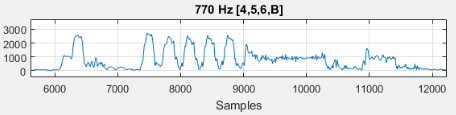
\includegraphics[scale=0.8]{Billeder/NoWindow.PNG}
\caption{Her ses magnitude på 770 Hz for et signal sendt med en tonelængde på 20 ms, uden en vinduefunktion på modtagersiden}
\label{fig:NoWindow}
\end{figure}

\begin{figure}[h]
\centering
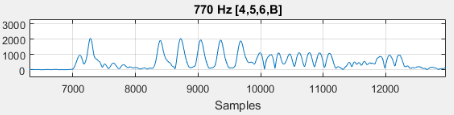
\includegraphics[scale=0.8]{Billeder/HannWindow.PNG}
\caption{Her ses magnitude på 770 Hz for samme signal sendt med en tonelængde på 20 ms, med et Hann-vindue på modtagersiden}
\label{fig:NoWindow}
\end{figure}

Signalet på billederne indeholder fem toner, hvor 770 Hz indgår. De steder hvor magnitude stiger til godt 50 \% af de store peaks, er der toner, hvor 697 Hz indgår. Det gør margenen, hvor man kan placere threshold ret lille - det er et problem der bliver værre jo kortere toner man sender. Typen af vinduefunktion gør ikke den store forskel, men forskellen fra at køre med og uden er ret markant. Det kan ses at man kan opleve spikes, hvor magnitude stiger op på et niveau, der ligger meget tæt på threshold. Det kan derfor konkluderes at det er nødvendigt at bruge en vinduefunktion, hvis man er interesseret i at sende korte toner.

\subsection{Hastighedstests}



\subsection{DTMF-tone transition}

